\textbf{Problema:} Seja $f:U\subseteq \mathbb{R}^{2}\to\mathbb{R}$ tal que $f(x,y)=c$. Quando podemos resolver esta equação para $y$ como função de $x$?
\begin{example}
  $$f(x,y)=x^{2}+y^{2}.$$
  Note que o gráfico de $f(x,y)=c$ é e seguinte 
  \begin{center}
    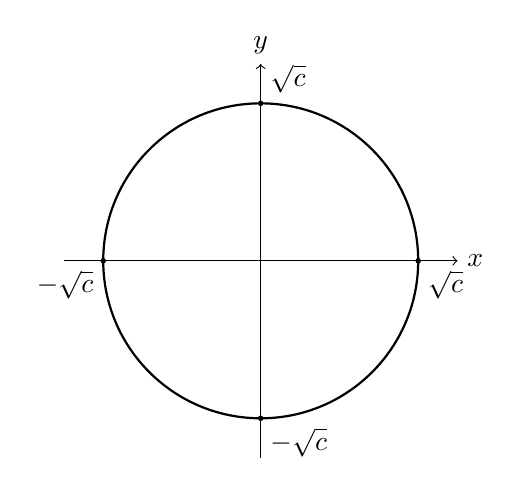
\begin{tikzpicture}[scale=1]

  % Definir el radio
  \def\r{2} % aquí puedes cambiar el valor (esto representa \sqrt{c})

  % Ejes
  \draw[->] (-\r-0.5,0) -- (\r+0.5,0) node[right] {$x$};
  \draw[->] (0,-\r-0.5) -- (0,\r+0.5) node[above] {$y$};

  % Circunferencia
  \draw[thick] (0,0) circle (\r);

  % Puntos de intersección con los ejes
  \fill (\r,0) circle (1pt) node[below right] {$\sqrt{c}$};
  \fill (-\r,0) circle (1pt) node[below left] {$-\sqrt{c}$};
  \fill (0,\r) circle (1pt) node[above right] {$\sqrt{c}$};
  \fill (0,-\r) circle (1pt) node[below right] {$-\sqrt{c}$};

\end{tikzpicture}

  
  \end{center}
  Suponha $c=1$, logo note que
  \begin{itemize}
    \item $\frac{\partial f}{\partial x}(0,1)=0$, logo no se pode resolver a $x$ en função de $y$.
    \item $\frac{\partial f}{\partial y}(0,1)=2\neq 0$, logo temos que $y=\sqrt{1-x^{2}}$.
  \end{itemize}
\end{example}
\begin{definition}[Hipersuperfície]
  Um $M\subseteq \mathbb{R}^{n+1}$ chama-se uma \textbf{hipersuperfície} de classe $C^{k}$ quando para cada $p\in M$ existe um aberto $V\subseteq \mathbb{R}^{n+1}$ e uma função $\xi:U\to\mathbb{R}$ com $U\subseteq\mathbb{R}^{n}$ aberto de classe $C^{k}$ taes que $p\in V$ e $V\cap M=\graf(\xi)$.\\
  Ou seja, para algúm inteiro $i\in\{1,\cdots,n+1\}$ ten-se que
  \begin{align*}
    V\cap M=\{(x_1,\cdots,x_{n+1})\in\mathbb{R}^{n+1}:x_i=\xi(x_1,\cdots,x_{i-1},x_{i+1},\cdots,x_n)\}.
  \end{align*}
\end{definition}
\begin{example}[$S^{n}$]
  Seja $S^{n}$ definido por
  \begin{align*}
    S^{n}=\{x\in\mathbb{R}^{n+1}:\left\langle x,x \right\rangle=1\}.
  \end{align*}
  Note que $S^{n}$ é uma hipersuperfície $C^{\infty}$.\\
  Defina para cada $i\in\{1,\cdots,n+1\}$ o seguinte
  \begin{itemize}
    \item $V_i=\{x\in\mathbb{R}^{n+1}:x_i>0\}$.
    \item $U_i=\{x\in\mathbb{R}^{n+1}:x_i<0\}$.
  \end{itemize}
  Escrevamos $x^{+}=(x_1,\cdots,x_{i-1},x_{i+1},\cdots,x_{n+1})$, logo
  \begin{itemize}
    \item $x\in S^{n}\cap V_i$ se, somente se $|x^{+}|<1$ e $x_i=\sqrt{1-|x^{+}|^{2}}$. 
    \item $x\in S^{n}\cap U_i$ se, somente se $|x^{+}|<1$ e $x_i=-\sqrt{1-|x^{+}|^{2}}$. 
  \end{itemize}
  Logo $S^{n}$ é uma hipersuperfície de classe $C^{\infty}$. 
\end{example}
\begin{definition}[Espaço vetorial Tangente]
  Seja $M$ uma hipersuperfície de classe $C^{k}$ ($k\geq 1$), para cada $p\in M$.\\
  Definimos o \textbf{espaço vetorial tangente} por
  \begin{align*}
    T_{p}M=\{v=\lambda^{\prime}(0):\lambda:(-\delta,\delta)\to M\text{ diferenciável com }\lambda(0)=p\}.
  \end{align*}
\end{definition}
\begin{definition}[Valor regular e nivel crtítico]
  Um número $c\in\mathbb{R}$ chama-se \textbf{valor regular} de uma função $f:U\subseteq \mathbb{R}^{n}\to\mathbb{R}$ de classe $C^{1}$ quando $f(x)=c$, implica que $\nabla f(x)\neq 0$.\\
  Se existe $x\in U$ com $f(x)=c$ e $\nabla f(x)=0$, $c$ é chamado \textbf{nivel crítico}. 
\end{definition}
\begin{theorem}[Teorema de função implícita]
  Sejam $U\subseteq \mathbb{R}^{n+m}=\mathbb{R}^{n}\times \mathbb{R}^{m}$ um aberto, $f:U\to\mathbb{R}^{m}$ uma aplicação de classe $C^k$ com $k\geq 1$ e $(a,b)\in U$ taes que $f(a,b)=c\in\mathbb{R}^{m}$. Nessão condições, se $f^{\prime}(a,b)\big|_{\{0\}\times\mathbb{R}^{m}}=\frac{\partial f}{\partial y}(a,b)$ é um isomorfismo sobre $\mathbb{R}^{m}$, então existen abertos $V$ com $(a,b)\in V$, $V\subseteq U$ e $A$ com $a\in A$ e $A\subseteq\mathbb{R}^{n}$ que cumpren
  \begin{enumerate}
    \item Para todo $x\in A$, existem um único $y=\xi(x)\in\mathbb{R}^{m}$ tal que $(x,\xi(x))\in V$ e $f(x,\xi(x))=c$.
    \item A aplicação $\xi:A\to\mathbb{R}^{m}$ é de classe $C^{k}$ e $\xi^{\prime}(a)=-T_2^{-1}T_1$, onde $T_1\in L(\mathbb{R}^{n},\mathbb{R}^{m})$ e $T_2\in L(\mathbb{R}^{m})$ são definidas por
      \begin{align*}
        T_1h&=f^{\prime}(a,b)\cdot (h,0).\\
        T_2h&=f^{\prime}(a,b)\cdot (0,h).
      \end{align*}
  \end{enumerate}
\end{theorem}
\begin{proof}
  \begin{center}
    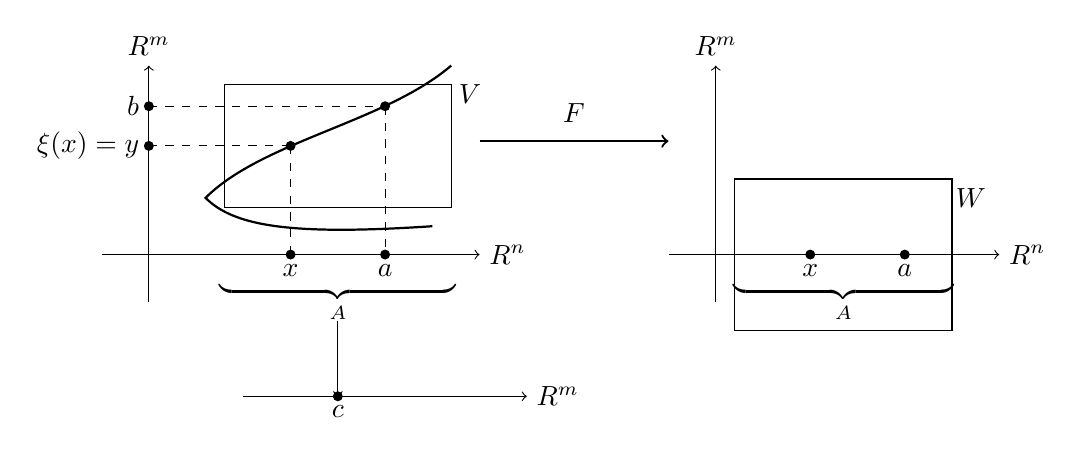
\begin{tikzpicture}[scale=1.2]

  % Ejes izquierda
  \draw[->] (-3,-0.5) -- (-3,2) node[above] {$\mathbb{R}^m$};
  \draw[->] (-3.5,0) -- (0.5,0) node[right] {$\mathbb{R}^n$};

  % Conjunto A (intervalo)
  \draw (-2,0) -- (0,0);
  \node at (-1,-0.5) {
    $\underbrace{\hspace{3cm}}_{A}$
  };

  % Puntos en A
  \fill (-1.5,0) circle (1.5pt) node[below] {$x$};
  \fill (-0.5,0) circle (1.5pt) node[below] {$a$};
  \fill (-0.5,1.57) circle (1.5pt);
  \fill (-1.5,1.15) circle (1.5pt);
  \fill (-3,1.57) circle (1.5pt) node[left] {$b$};
  \fill (-3,1.15) circle (1.5pt) node[left] {$\xi(x)=y$};
  \draw[dashed] (-3,1.57) -- (-0.5,1.57);
  \draw[dashed] (-0.5,1.57) -- (-0.5,0);
  \draw[dashed] (-3,1.15) -- (-1.5,1.15);
  \draw[dashed] (-1.5,1.15) -- (-1.5,0);
  
  % Rectángulo (V)
  \draw (-2.2,0.5) rectangle (0.2,1.8);
  \node at (0.4,1.7) {$V$};
  
  % Curva dentro
      \draw[thick] 
      (0,0.3) 
      .. controls (-1.5,0.2) and (-2.1,0.3) .. (-2.4,0.6)
      .. controls (-1.8,1.2) and (-0.5,1.4) .. (0.2,2);
  
  % Flecha F
  \draw[->, thick] (0.5,1.2) to[out=0,in=180] (2.5,1.2);
  \node at (1.5,1.5) {$F$};
  
  % Ejes derecha
  \draw[->] (3,-0.5) -- (3,2) node[above] {$\mathbb{R}^m$};
  \draw[->] (2.5,0) -- (6,0) node[right] {$\mathbb{R}^n$};
  
  
  % Rectángulo (W)
  \draw (3.2,-0.8) rectangle (5.5,0.8);
  \node at (5.7,0.6) {$W$};
  
  % Conjunto A (intervalo)
  \draw (-2,0) -- (0,0);
  \node at (4.35,-0.5) {
      $\underbrace{\hspace{2.8cm}}_{A}$
  };
  
  % Puntos imagen
  \fill (4,0) circle (1.5pt) node[below] {$x$};
  \fill (5,0) circle (1.5pt) node[below] {$a$};
  
  % Flecha hacia abajo (A a c)
  \draw[->] (-1,-0.7) -- (-1,-1.5);
  
  % Línea inferior
  \draw (-2,-1.5) -- (0,-1.5);
  \fill (-1,-1.5) circle (1.5pt) node[below] {$c$};
  \draw[->] (0,-1.5) -- (1,-1.5) node[right] {$\mathbb{R}^m$};

\end{tikzpicture}
  
  \end{center}
  Sem perdida de generalidade considere $c=0$.\\
  Considere $F:U\to\mathbb{R}^{n}\times\mathbb{R}^{m}$ definida por $F(x,y)=(x,f(x,y))$.\\
  Logo $F$ é $C^{k}$, assim
  \begin{align*}
    F^{\prime}(a,b)\cdot (h,k)=(h,f^{\prime}(a,v)\cdot(h,k)).
  \end{align*}
  Onde $(h,k)\in\mathbb{R}^{n}\times\mathbb{R}^{m}$.\\
  Se $F^{\prime}(a,b)\cdot(h,k)=(0,0)$, então temos que $h=0$.\\
  Logo, como $f\big|_{\{0\}\times\mathbb{R}^{m}}$ é um isomoorfismo, $F^{\prime}(a,b)\cdot (0,k)=0$ implica que $k=0$.\\
  Portanto, $F^{\prime}(a,b)$ é injetiva e como é  uma aplicação linear entre espaços da mesma dimensão, é um isomorfismo de $\mathbb{R}^{n}\times\mathbb{R}^{m}$ sobre si mesmo.\\
  Assim, pelo teorema de la aplicação inversa temos que existen $V\subseteq U$ tal que $(a,b)\in V$ e $W\subseteq \mathbb{R}^{n}\times\mathbb{R}^{m}$ tal que $F(a,b)=(a,0)\in W$ e $W=A\times B$ com $A\subseteq \mathbb{R}^{n}$ e $B\subseteq \mathbb{R}^{m}$ abertos, taes que $F\big|_{V}:V\to W$ é um $C^{k}$-difeomorfismo.\\
  Logo, para cada $x\in A$, com $(x,0)\in W$ existe um único $(x,y)\in V$ tal que $F(x,y)=(x,0)$. Definimos $\xi(x)=y$. Assim, para cada $x\in A$ temos que $f(x,\xi(x))=c=0$.
  \begin{itemize}
    \item Regularidade de $\xi$.\\
      Consideremos $G=\left[ F\big|_{V} \right]^{-1}$ a qual é $C^{k}$ pelo teorema de la aplicação inversa, logo temos que $G(x,0)=(x,\xi(x))$.\\
      Assim, definindo $\varphi(x)=(x,0)$ que é $C^{\infty}$ e a projeção $p_2(x,y)=2$, obtemos que $\xi=p_2\circ G\circ \varphi \in C^{k}$.
    \item Fórmula de la derivada.\\
      Sabemos que, para todo $(h,k)\in\mathbb{R}^{n}\times\mathbb{R}^{m}$ se cumpre que
      \begin{align*}
        f^{\prime}(a,b)\cdot (h,k)=f^{\prime}(a,b)\cdot(h,0)+f^{\prime}(a,b)\cdot (0,k)=T_1\cdot h+T_2\cdot k.
      \end{align*}
      Como $f(x,\xi(x))=0$, temos que $f^{\prime}(a,\xi(a))\cdot(h,\xi^{\prime}(a))=0$, pela regra da cadeia, logo
      \begin{align*}
        0&=f^{\prime}(a,\xi(a))\cdot(h,\xi^{\prime}(a)\cdot h)\\
        &=f^{\prime}(a,\xi(a))\cdot(h,0)+f^{\prime}(a,\xi(a))\cdot(0,\xi^{\prime}(a)\cdot h)\\
        &=T_1\cdot h+T_2\cdot\xi^{\prime}(a)\cdot h.
      \end{align*}
      Assim
      \begin{align*}
        \xi^{\prime}(a)&=-T_2^{-1}\circ(T_1)\\
        &=-\left( \frac{\partial f}{\partial y}(a,b) \right)^{-1}\cdot\left( \frac{\partial f}{\partial x}(a,b)\cdot h \right).
      \end{align*}
  \end{itemize}
\end{proof}
